\documentclass[a4paper, 10pt, danish, final]{article}
\usepackage{bonde}

\def\mytitle{Dataanalyse 2010}
\def\mysubtitle{Aflevering af ugeopgave 2}
\def\myauthor{Ulrik Bonde}
\def\mymail{\mailto{bonde@diku.dk}}
\def\mydate{\today}
\def\repository{\url{http://github.com/bonde/dataanalyse}}

\title{\mytitle}
\subtitle{\mysubtitle}

\author{\myauthor{} - \mymail}
\date{\mydate}

\hypersetup{
colorlinks,%
citecolor=black,%
filecolor=black,%
linkcolor=black,%
urlcolor=black,%
bookmarksopen=false,
pdftitle={\mytitle{} - \mysubtitle},
pdfauthor={\myauthor}
}

\begin{document}
\maketitle

\subsection*{Spørgsmål 1}
Jeg vil i denne opgave bruge et meget simpelt billede til at illustrere
den to-dimensionelle Fouriertransformation og effekten af ideel
filtrering af billeder. Billedet er vist i figur \ref{square} og er en
hvid firkant på en sort baggrund.

\begin{figure}[!h]
    \centering
    
\includegraphics[angle=0,width=0.45\textwidth]{images/square}
    \caption[]{Billedet som vi vil arbejde med. Motivet et simpelt og
    der er skarpe kontraster.}
    \label{square}
\end{figure}

Vi vil nu gerne finde billedets Fouriertransformation og vise det med og
uden translation af Origo til billedets midte. Fremgangsmåden er vist i
kodeboks \ref{fft_matlab} og de resulterende billeder er vist i figur
\ref{ffts}. Der ses

\begin{lstlisting}[caption={Fouriertransformation i MATLAB},
    captionpos=b, label={fft_matlab}, float=t, numbers=none]
% Read and show the original image
[I, cmap] = imread('../images/square.tiff', 'tiff');
figure; imshow(I, cmap);

% Show Fourier transform without shift
figure; imshow(log(abs(fft2(I))), cmap);

% Show Fourier transform with shift
figure; imshow(log(abs(fftshift(fft2(I)))), cmap);
\end{lstlisting}

\begin{figure}[!h]
    \centering
    \subfloat[Styrkespektret uden translation af Origo]{\label{fft_noshift}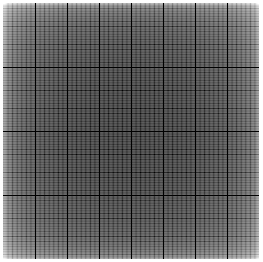
\includegraphics[angle=0,width=0.45\textwidth]{images/fft_noshift}\hspace{1em}}
    \subfloat[Styrkespektret med translation af Origo til
    billedecenteret]{\label{fft_shift}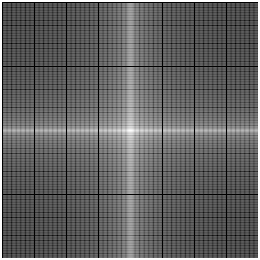
\includegraphics[angle=0,width=0.45\textwidth]{images/fft_shift}}
    \caption[]{To forskellige visninger af den samme
    Fouriertransformation. Billedet til venstre viser det egentlige
    output fra metoden \texttt{fft2} i MATLAB. Billedet til højre er
    blevet justeret således at vi har Origo i billedets midte.
    Billederne er lavet som vist i kodeboks \ref{fft_matlab}.}
    \label{ffts}
\end{figure}

\subsection*{Spørgsmål 2}


%%%%%%%%%%%%%%%%%%%%%%%%%%%%%%%%%%%%%%%%%%%%%%%%%%%%%%%%%%%%%%%%%%%%
% Formal stuff

%\bibliographystyle{abbrvnat}
%\bibliography{bibliography}
%\addcontentsline{toc}{chapter}{Litteratur}

\clearpage
\appendix
\lstset{language=Matlab, basicstyle=\scriptsize,
    showstringspaces=false, numbers=left, stepnumber=1,
    numberstyle=\tiny, frame=none}
\section{Kildekode}
Kildekoden er tilgængelig i mit git-repository på \repository{}. Bemærk
at prefikset \texttt{DA} står for ``DataAnalyse'' og blot er til for at
undgå eventuelle sammenstød med indbyggede funktioner i MATLAB.

\subsection{DAIdealFilter.m}
\lstinputlisting{../src/DAIdealFilter.m}

\subsection{DAFilterF.m}
\lstinputlisting{../src/DAFilterF.m}

\end{document}

% vim: set tw=72 spell spelllang=da:
